\documentclass[12pt,letterpaper]{article}

\usepackage[utf8]{inputenc}
\usepackage[T1]{fontenc}
\usepackage[english]{babel}
\usepackage{amsmath, amssymb, amsthm}
\usepackage{float, enumitem, xcolor, geometry}
\usepackage{graphicx, fancyhdr, fancyvrb}
\usepackage{array, makecell}
\usepackage{forest}
\usepackage[normalem]{ulem}
\usepackage[colorlinks=true, linkcolor=linkblue, urlcolor=linkblue, citecolor=linkblue]{hyperref}
\usepackage{makecell}
\usepackage{tikz}
\usetikzlibrary{automata, positioning, arrows.meta}

\definecolor{linkblue}{HTML}{1A167A}

\geometry{margin=2cm, top=2cm, bottom=2cm}

\newcommand{\pred}{$\rightarrow$}
\newcommand{\asig}{$\leftarrow$}

% ========================================
% COLORES
% ========================================
\definecolor{green_checkmark}{HTML}{07E314}
\definecolor{red_cross}{HTML}{ED4728}

% ========================================
% COMANDOS PARA MARCADORES
% ========================================
\newcommand{\greencheck}{\textcolor{green_checkmark}{$\checkmark$}}
\newcommand{\redcross}{\textcolor{red_cross}{$\times$}}

% ========================================
% CONSTANTES DEL ENCABEZADO
% ========================================
\newcommand{\encabezadoIzq}{Compiladores 2027-1}
\newcommand{\encabezadoCen}{Tarea 2}
\newcommand{\encabezadoDer}{\textit{Minim, deriv, elim y EBNF}}

% ========================================
% CONFIGURACION DEL ENCABEZADO
% ========================================
\pagestyle{fancy}
\fancyhf{}

\fancyhead[L]{\encabezadoIzq}
\fancyhead[C]{\encabezadoCen}
\fancyhead[R]{\encabezadoDer}

\fancyfoot[C]{\thepage}

\renewcommand{\headrulewidth}{0.1pt}
\renewcommand{\footrulewidth}{0pt}

% ========================================
% CONFIGURACION DE TABLAS
% ========================================
\newcolumntype{C}[1]{>{\centering\arraybackslash}m{#1}}
\newcolumntype{L}[1]{>{\raggedright\arraybackslash}m{#1}}
\newcolumntype{R}[1]{>{\raggedleft\arraybackslash}m{#1}}

\begin{document}

\thispagestyle{empty}
\begin{titlepage}
  \thispagestyle{empty}
  %--------------- COMANDO LINEA----------------->
  \newcommand{\linea}{\rule{\linewidth}{0.5mm}}                 
  \center
  %<<<<<<<<<<<<<<<<<<<<<<<<<<<<<<<<<<<<<<<<<<<

  %Add logos
  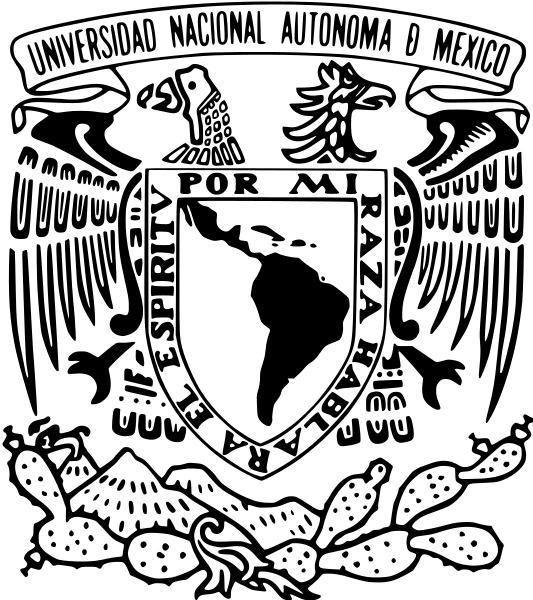
\includegraphics[width=0.24\textwidth]{../unam_logo.png} \hspace{1.5cm}
  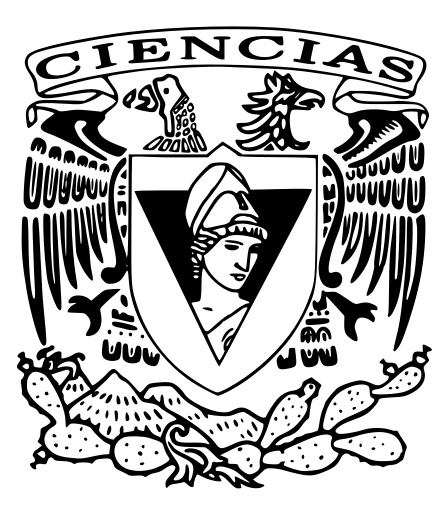
\includegraphics[width=0.25\textwidth]{../fc_logo.png} \\[1cm]
  \textbf{\Large UNIVERSIDAD NACIONAL AUTÓNOMA}\\[3mm]
  \textbf{\Large DE MÉXICO} \\[6mm]
  \textit{\Large Facultad de Ciencias}

  \vfill

  %---------------TÍTULO----------------->
  \linea
  \vfill \vspace{1cm}
  \textbf{\Large Compiladores}\\[1.1cm]
  \textbf{\Large Minimización, derivación, eliminación\\[0.2cm] de ambigüedades y notación EBNF}\\[0.9cm]
  \linea \\
  \vfill
  \vspace{0.7cm}
  %Title of the Research
  \textbf{\Large  Tarea 2}\\[6mm]
  %<<<<<<<<<<<<<<<<<<<<<<<<<<<<<<<<<<<<<<<<<<<

  %Team
  \vfill
  \textit{\small Presenta:}\\
  \textbf{\large  \textbf{Ramírez Juárez María Fernanda} - 321204747}\\[3mm]
  \textbf{\large  \textbf{Rojo Peña Manuel Ianluck} - 118005762}\\[3mm]

  %Profesor y Grupo
  \textit{\small Profesor:}\\
  \textbf{Pablo Martínez Yessica Janeth}\\[3mm]
  \textit{\small Ayudante:}\\
  \textbf{Rojas Fuentes Andrea}\\[3mm]
  \small Grupo: 7010, 2027-1\\[3mm]
  \vfill

  %Fecha or Date
  \textit{\small Fecha de entrega:}\\
         {\large 14 de septiembre, 2026}
         
\end{titlepage}


%%%%%%%%%%%%%%%%%%%%%%%%%%%%%%%%%%%%%%%%%%
\newpage
%%%%%%%%%%%%%%%%%%%%%%%%%%%%%%%%%%%%%%%%%%

\begin{enumerate}[label=\arabic*.]

\item Dada la tabla de transiciones de un AFD:

  \[
  \begin{array}{c|cc}
    & 0 & 1 \\ \hline
    \rightarrow A & B & E \\
    B & C & F \\
    * C & D & H \\
    D & E & H \\
    E & F & I \\
    * F & G & B \\
    G & H & B \\
    H & I & C \\
    * I & A & E
  \end{array}
  \]

  \begin{enumerate}
  \item Obtén el AFD equivalente con el mínimo número de estados.
  \end{enumerate}

  \bigskip

  \subsubsection*{Paso 1. Partición inicial}
  Dividimos los estados según sean de aceptación o no:
  \[
  \alpha = \{C,\, F,\, I\} \qquad \beta = \{A,\, B,\, D,\, E,\, G,\, H\}
  \]

  \subsubsection*{Paso 2. Verificar transiciones dentro de cada grupo}
  Para cada estado, vemos a qué grupo ($\alpha$ o $\beta$) llegan sus transiciones con 0 y 1:

  \[
  \begin{array}{c|cc}
    \alpha & 0 & 1 \\ \hline
    C & \beta & \beta \\
    F & \beta & \beta \\
    I & \beta & \beta
  \end{array}
  \qquad
  \begin{array}{c|cc}
    \beta & 0 & 1 \\ \hline
    A & \beta & \beta \\
    B & \alpha & \alpha \\
    D & \beta & \beta \\
    E & \alpha & \alpha \\
    G & \beta & \beta \\
    H & \alpha & \alpha
  \end{array}
  \]

  \subsubsection*{Paso 3. Refinar la partición}
  Los estados de $\alpha$ se comportan igual entre sí (tienen las mismas transiciones), pero $\beta$ se divide: $\{A,D,G\}$ va a $(\beta,\beta)$ mientras que $\{B,E,H\}$ va a $(\alpha,\alpha)$. Renombramos:
  \[
  \alpha = \{C,\, F,\, I\} \qquad \beta = \{A,\, D,\, G\} \qquad \gamma = \{B,\, E,\, H\}
  \]

  \subsubsection*{Paso 4. Repetir la verificación con 3 grupos}
  \[
  \begin{array}{c|cc}
    \alpha & 0 & 1 \\ \hline
    C & \beta & \gamma \\
    F & \beta & \gamma \\
    I & \beta & \gamma
  \end{array}
  \qquad
  \begin{array}{c|cc}
    \beta & 0 & 1 \\ \hline
    A & \gamma & \gamma \\
    D & \gamma & \gamma \\
    G & \gamma & \gamma
  \end{array}
  \qquad
  \begin{array}{c|cc}
    \gamma & 0 & 1 \\ \hline
    B & \alpha & \alpha \\
    E & \alpha & \alpha \\
    H & \alpha & \alpha
  \end{array}
  \]

  \subsubsection*{Paso 5. Conclusión}
  Ya no se generan subgrupos nuevos, así que la partición es estable. El AFD mínimo tiene 3 estados:
  \[
  \alpha = \{C,F,I\} \quad (\text{de aceptación}) \qquad
  \beta = \{A,D,G\} \quad (\text{inicial}) \qquad
  \gamma = \{B,E,H\}
  \]

  \medskip

  \[
  \begin{array}{c|cc}
    & 0 & 1 \\ \hline
    \rightarrow \beta & \gamma & \gamma \\
    \gamma & \alpha & \alpha \\
    * \alpha & \beta & \gamma
  \end{array}
  \]
  
  \bigskip
  
  \begin{center}
    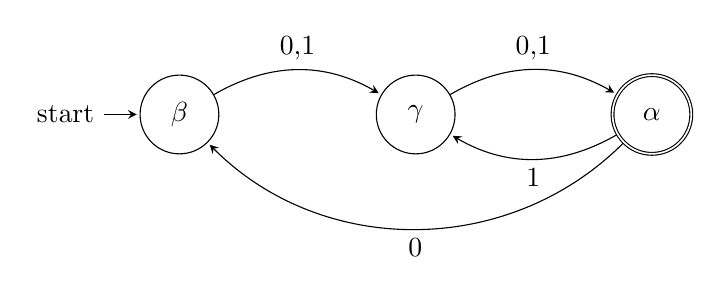
\begin{tikzpicture}[
        shorten >=1pt,
        node distance=3cm,
        auto,
        >=stealth,
        every state/.style={
          draw,
          circle,
          minimum size=1cm
        }
      ]
      \node[state, initial] (B) {$\beta$};
      \node[state, right of=B] (G) {$\gamma$};
      \node[state, accepting, right of=G] (A) {$\alpha$};

      \path[->]
      (B) edge[bend left]    node {0,1} (G)
      (G) edge[bend left]    node {0,1} (A)
      (A) edge[bend left]    node {1}   (G)
      (A) edge[bend left=45] node {0}   (B);
    \end{tikzpicture}
  \end{center}
  
  
%%%%%%%%%%%%%%%%%%%%%%%%%%%%%%%%%%%%%%%%%%
\newpage
%%%%%%%%%%%%%%%%%%%%%%%%%%%%%%%%%%%%%%%%%%

\item Usando el algoritmo de elementos punteados, construya los AFDs con el mínimo número de estados para las siguientes expresiones regulares.
  
  \begin{enumerate}
    
  \item $(a|b)^*a(a|b)$.

    \subsection*{Elementos Punteados}
    \textbf{Cerradua}\big(\{ r $\to$ $\bullet$ b(b $\mid$ aa$^*$b)c\}\big): como se trata de $*$,
    podemos expandir hacia sus dos alternativas \emph{o} ignorarlo y seguir con lo que está después del $*$:
      
    \medskip

    \textbf{Estado:}
    \[
    \begin{aligned}
      q_0 = \{\,
      r &\to (\bullet a\mid b)^*a(a\mid b),\\
      r &\to (a\mid \bullet b)^*a(a\mid b),\\
      r &\to (a\mid b)^*\bullet a(a\mid b)
      \,\}
    \end{aligned}
    \]
    
    \textbf{Transiciones:}
    \[
    \begin{aligned}
      \texttt{goto}(q_0, a) =
        \{\,
        r &\to(a\bullet\mid b)^*a(a\mid b),\\
        r &\to(a\mid b)^*\bullet a(a\mid b),\\
        r &\to\bullet(a\mid b)^* a(a\mid b)
        \,\} = Cerradura(q_0) \\
      &\cup\\
        \{\,
        r &\to(a\mid b)^*a\bullet(a\mid b)
        \,\} = \boxed{q_1}
    \end{aligned}
    \]

    \[
    \begin{aligned}
      \texttt{goto}(q_0, b) =
      \{\,
      r &\to(a\mid b\bullet)^*a(a\mid b),\\
      r &\to(a\mid b)^*\bullet a(a\mid b),\\
      r &\to\bullet(a\mid b)^* a(a\mid b)
      \,\} = \boxed{q0}
    \end{aligned}
    \]
    
    \medskip
  
  \textbf{Estado:}
  \[
  \begin{aligned}
    q_1 = &Cerradura(q_0) \cup
    \{\,
    r &\to(a\mid b)^*a\bullet(a\mid b),\\
    r &\to(a\mid b)^*a(\bullet a\mid b),\\
    r &\to(a\mid b)^*a(a\mid \bullet b)
    \,\}
  \end{aligned}
  \]

  \textbf{Transiciones:}
  \[
  \begin{aligned}
    \texttt{goto}(q_1, a) = &q_1 \cup\\
    \{\,
    r &\to(a\mid b)^*a(a\bullet\mid b),\\
    r &\to(a\mid b)^*a(a\mid b)\bullet
    \,\} = \boxed{q_2}
  \end{aligned}
  \]
  \[
  \begin{aligned}
    \texttt{goto}(q_1, b) = &q_0 \cup\\
    \{\,
    r &\to(a\mid b\bullet)^*a(a\mid b),\\
    r &\to(a\mid b)^*a(a\mid b\bullet),\\
    r &\to(a\mid b)^*a(a\mid b)\bullet
    \,\} = \boxed{q_3}\\
  \end{aligned}
  \]

  \medskip
  
  \textbf{Estado:}
  \[
  \begin{aligned}
    q_2 = &q_1 \cup\\
    \{\,
    r &\to(a\mid b)^*a(a\bullet\mid b),\\
    r &\to(a\mid b)^*a(a\mid b)\bullet
    \,\}
  \end{aligned}
  \]

  Es etado de acpetación.
  
  \bigskip
  
  \textbf{Transiciones:} Las hojas activas de $q_2$ son las mismas que las de $q_1$ (los ítems nuevos ya
  no tienen símbolo pendiente), así que:
  \[
  \texttt{goto}(q_2, a) = q_2
  \qquad
  \texttt{goto}(q_2, b) = q_3
  \]
  
  \medskip
  
  \textbf{Estado:}
  \[
  \begin{aligned}
    q_3 = &q_0 \cup\\
    \{\,
    r &\to(a\mid b\bullet)^*a(a\mid b),\\
    r &\to(a\mid b)^*a(a\mid b\bullet),\\
    r &\to(a\mid b)^*a(a\mid b)\bullet
    \,\} = \boxed{q_3}
  \end{aligned}
  \]

  Es estado de aceptación.

  \textbf{Transiciones:} las hojas activas de $q_3$ coinciden con las de $q_0$
  \[
  \texttt{goto}(q_3, a) = q_1
  \qquad
  \texttt{goto}(q_3, b) = q_0
  \]
  
  \bigskip
  
  \subsubsection*{Tabla de transiciones}
  \[
  \begin{array}{c|cc}
    & a & b \\ \hline
    \rightarrow q_0 & q_1 & q_0 \\
    q_1 & q_2 & q_3  \\
    {}^*q_2 & q_2 & q_3 \\
    {}^*q_3 & q_1 & q_0 \\
  \end{array}
  \]

  \medskip

  \subsection*{Minimización}

  \subsubsection*{Paso 1. Partición inicial}
  \[
  \alpha = \{q_2,\, q_3\} \qquad \beta = \{q_0,\, q_1\}
  \]

  \subsubsection*{Paso 2. Verificar transiciones dentro de cada grupo}
  \[
  \begin{array}{c|cc}
    \alpha & a & b \\ \hline
    q_2 & \alpha & \alpha \\
    q_3 & \beta & \beta
  \end{array}
  \qquad
  \begin{array}{c|cc}
    \beta & a & b \\ \hline
    q_0 & \beta & \beta \\
    q_1 & \alpha & \alpha
  \end{array}
  \]

  \subsubsection*{Paso 3. Refinar la partición}
  En $\alpha$, $q_2$ se comporta como $(\alpha,\alpha)$ mientras que $q_3$ se comporta como $(\beta,\beta)$: se separan.
  En $\beta$, $q_0$ se comporta como $(\beta,\beta)$ mientras que $q_1$ se comporta como $(\alpha,\alpha)$: también se separan.

  \[
  \alpha = \{q_2\} \qquad \beta = \{q_0\} \qquad \gamma = \{q_1\} \qquad \delta = \{q_3\}
  \]

  \subsubsection*{Paso 4. Conclusión}
  Los cuatro grupos son unitarios: ya no pueden refinarse más. No existen estados equivalentes, por lo que \textbf{el AFD ya era mínimo} (4 estados).

  \medskip

  \[
  \begin{array}{c|cc}
    & a & b \\ \hline
    \rightarrow q_0 & q_1 & q_0 \\
    q_1 & q_2 & q_3 \\
    {}^*q_2 & q_2 & q_3 \\
    {}^*q_3 & q_1 & q_0 \\
  \end{array}
  \]

  \bigskip

    \begin{center}
    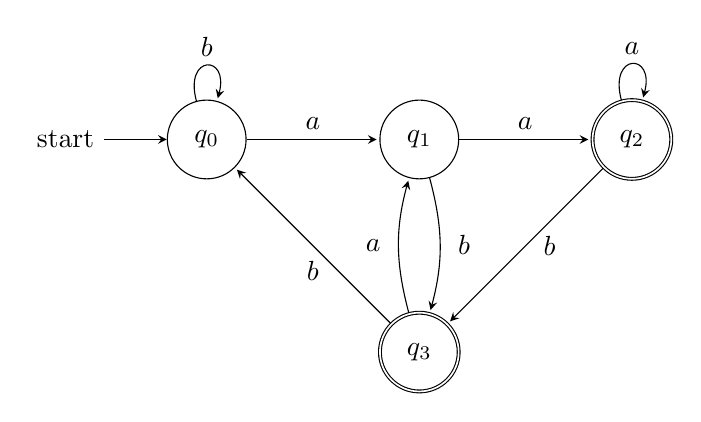
\begin{tikzpicture}[
        >=stealth,
        node distance=2.7cm,
        auto,
        every state/.style={
          draw,
          circle,
          minimum size=1cm,
          inner sep=2pt
        }
      ]

      % Estados
      \node[state, initial, initial distance=8mm] (q0) {$q_0$};
      \node[state, right of=q0] (q1) {$q_1$};
      \node[state, accepting, right of=q1] (q2) {$q_2$};
      \node[state, accepting, below of=q1] (q3) {$q_3$};

      % Transiciones
      \path[->, shorten >=1pt]
      % q0
      (q0) edge[loop above, looseness=6]
      node {$b$} (q0)

      (q0) edge
      node {$a$} (q1)

      % q1
      (q1) edge
      node {$a$} (q2)

      (q1) edge[bend left=15]
      node[right=3pt] {$b$} (q3)

      % q2
      (q2) edge[loop above, looseness=6]
      node {$a$} (q2)

      (q2) edge
      node[right=3pt] {$b$} (q3)

      % q3
      (q3) edge[bend left=15]
      node[left=3pt] {$a$} (q1)

      (q3) edge[right=35]
      node[below=2pt] {$b$} (q0);

    \end{tikzpicture}
  \end{center}
  
  \newpage
  
\item $(a|b)^*a(a|b)(a|b)$.

  \subsection*{Elementos Punteados}
  Se construye igual que en el anterior, solo se agrega un grupo $(a\mid b)$ más al final. Por brevedad
  listamos los estados de forma compacta (mismo procedimiento de cerradura/\texttt{goto}):
  
  \[
  \begin{aligned}
    q_0 &= \{\, (\bullet a\mid b)^*a(a\mid b)(a\mid b),\;(a\mid\bullet b)^*a(a\mid b)(a\mid b),\;(a\mid b)^*\bullet a(a\mid b)(a\mid b) \,\} \\
    q_1 &= q_0 \cup \{\, (a\mid b)^*a(\bullet a\mid b)(a\mid b),\;(a\mid b)^*a(a\mid\bullet b)(a\mid b) \,\} \\
    q_2 &= q_1 \cup \{\, (a\mid b)^*a(a\mid b)(\bullet a\mid b),\;(a\mid b)^*a(a\mid b)(a\mid\bullet b) \,\} \\
    q_3 &= q_0 \cup \{\, (a\mid b)^*a(a\mid b)(\bullet a\mid b),\;(a\mid b)^*a(a\mid b)(a\mid\bullet b) \,\} \\
    q_4 &= q_2 \cup \{\, (a\mid b)^*a(a\mid b)(a\mid b)\bullet \,\} \text{  Estado de aceptación} \\
    q_5 &= q_3 \cup \{\, (a\mid b)^*a(a\mid b)(a\mid b)\bullet \,\} \text{  Estado de aceptación} \\
    q_6 &= q_1 \cup \{\, (a\mid b)^*a(a\mid b)(a\mid b)\bullet \,\} \text{  Estado de aceptación} \\
    q_7 &= q_0 \cup \{\, (a\mid b)^*a(a\mid b)(a\mid b)\bullet \,\} \text{  Estado de aceptación}
  \end{aligned}
  \]

  \subsubsection*{Tabla de transiciones}
    \[
    \begin{array}{c|cc}
      & a & b \\ \hline
      \rightarrow q_0 & q_1 & q_0 \\
      q_1 & q_2 & q_3 \\
      q_2 & q_4 & q_5 \\
      q_3 & q_6 & q_7 \\
      {}^*q_4 & q_4 & q_5 \\
      {}^*q_5 & q_6 & q_7 \\
      {}^*q_6 & q_2 & q_3 \\
      {}^*q_7 & q_1 & q_0
    \end{array}
    \]

    \medskip
    
    \subsection*{Minimización}

    \subsubsection*{Paso 1. Partición inicial}
    \[
    \alpha = \{q_4,q_5,q_6,q_7\} \qquad \beta = \{q_0,q_1,q_2,q_3\}
    \]

    \subsubsection*{Paso 2. Verificar transiciones dentro de cada grupo}
    \[
    \begin{array}{c|cc}
      \alpha & a & b \\ \hline
      q_4 & \alpha & \alpha \\
      q_5 & \alpha & \alpha \\
      q_6 & \beta & \beta \\
      q_7 & \beta & \beta
    \end{array}
    \qquad
    \begin{array}{c|cc}
      \beta & a & b \\ \hline
      q_0 & \beta & \beta \\
      q_1 & \beta & \beta \\
      q_2 & \alpha & \alpha \\
      q_3 & \alpha & \alpha
    \end{array}
    \]

    \subsubsection*{Paso 3. Refinar la partición}
    \[
    \alpha = \{q_4,q_5\} \qquad \beta = \{q_0,q_1\} \qquad \gamma = \{q_6,q_7\} \qquad \delta = \{q_2,q_3\}
    \]

    \subsubsection*{Paso 4. Repetir la verificación con 4 grupos}
    \[
    \begin{array}{c|cc}
      \alpha & a & b \\ \hline
      q_4 & \alpha & \alpha \\
      q_5 & \gamma & \gamma
    \end{array}
    \qquad
    \begin{array}{c|cc}
      \beta & a & b \\ \hline
      q_0 & \beta & \beta \\
      q_1 & \delta & \delta
    \end{array}
    \]
    \[
    \begin{array}{c|cc}
      \gamma & a & b \\ \hline
      q_6 & \delta & \delta \\
      q_7 & \beta & \beta
    \end{array}
    \qquad
    \begin{array}{c|cc}
      \delta & a & b \\ \hline
      q_2 & \alpha & \alpha \\
      q_3 & \gamma & \gamma
    \end{array}
    \]

    \subsubsection*{Paso 5. Refinar de nuevo}
    Cada uno de los cuatro grupos se separa en dos, dando 8 grupos unitarios:
    \[
    \{q_4\},\{q_5\},\{q_6\},\{q_7\},\{q_0\},\{q_1\},\{q_2\},\{q_3\}
    \]

    \subsubsection*{Paso 6. Conclusión}
    Ya no es posible refinar más (todos los grupos son unitarios). No existen estados equivalentes: \textbf{el AFD ya era mínimo} (8 estados).

    \medskip

    \[
    \begin{array}{c|cc}
      & a & b \\ \hline
      \rightarrow q_0 & q_1 & q_0 \\
      q_1 & q_2 & q_3 \\
      q_2 & q_4 & q_5 \\
      q_3 & q_6 & q_7 \\
      {}^*q_4 & q_4 & q_5 \\
      {}^*q_5 & q_6 & q_7 \\
      {}^*q_6 & q_2 & q_3 \\
      {}^*q_7 & q_1 & q_0 \\
    \end{array}
    \]

    \bigskip

    \begin{figure}[H]
      \centering
      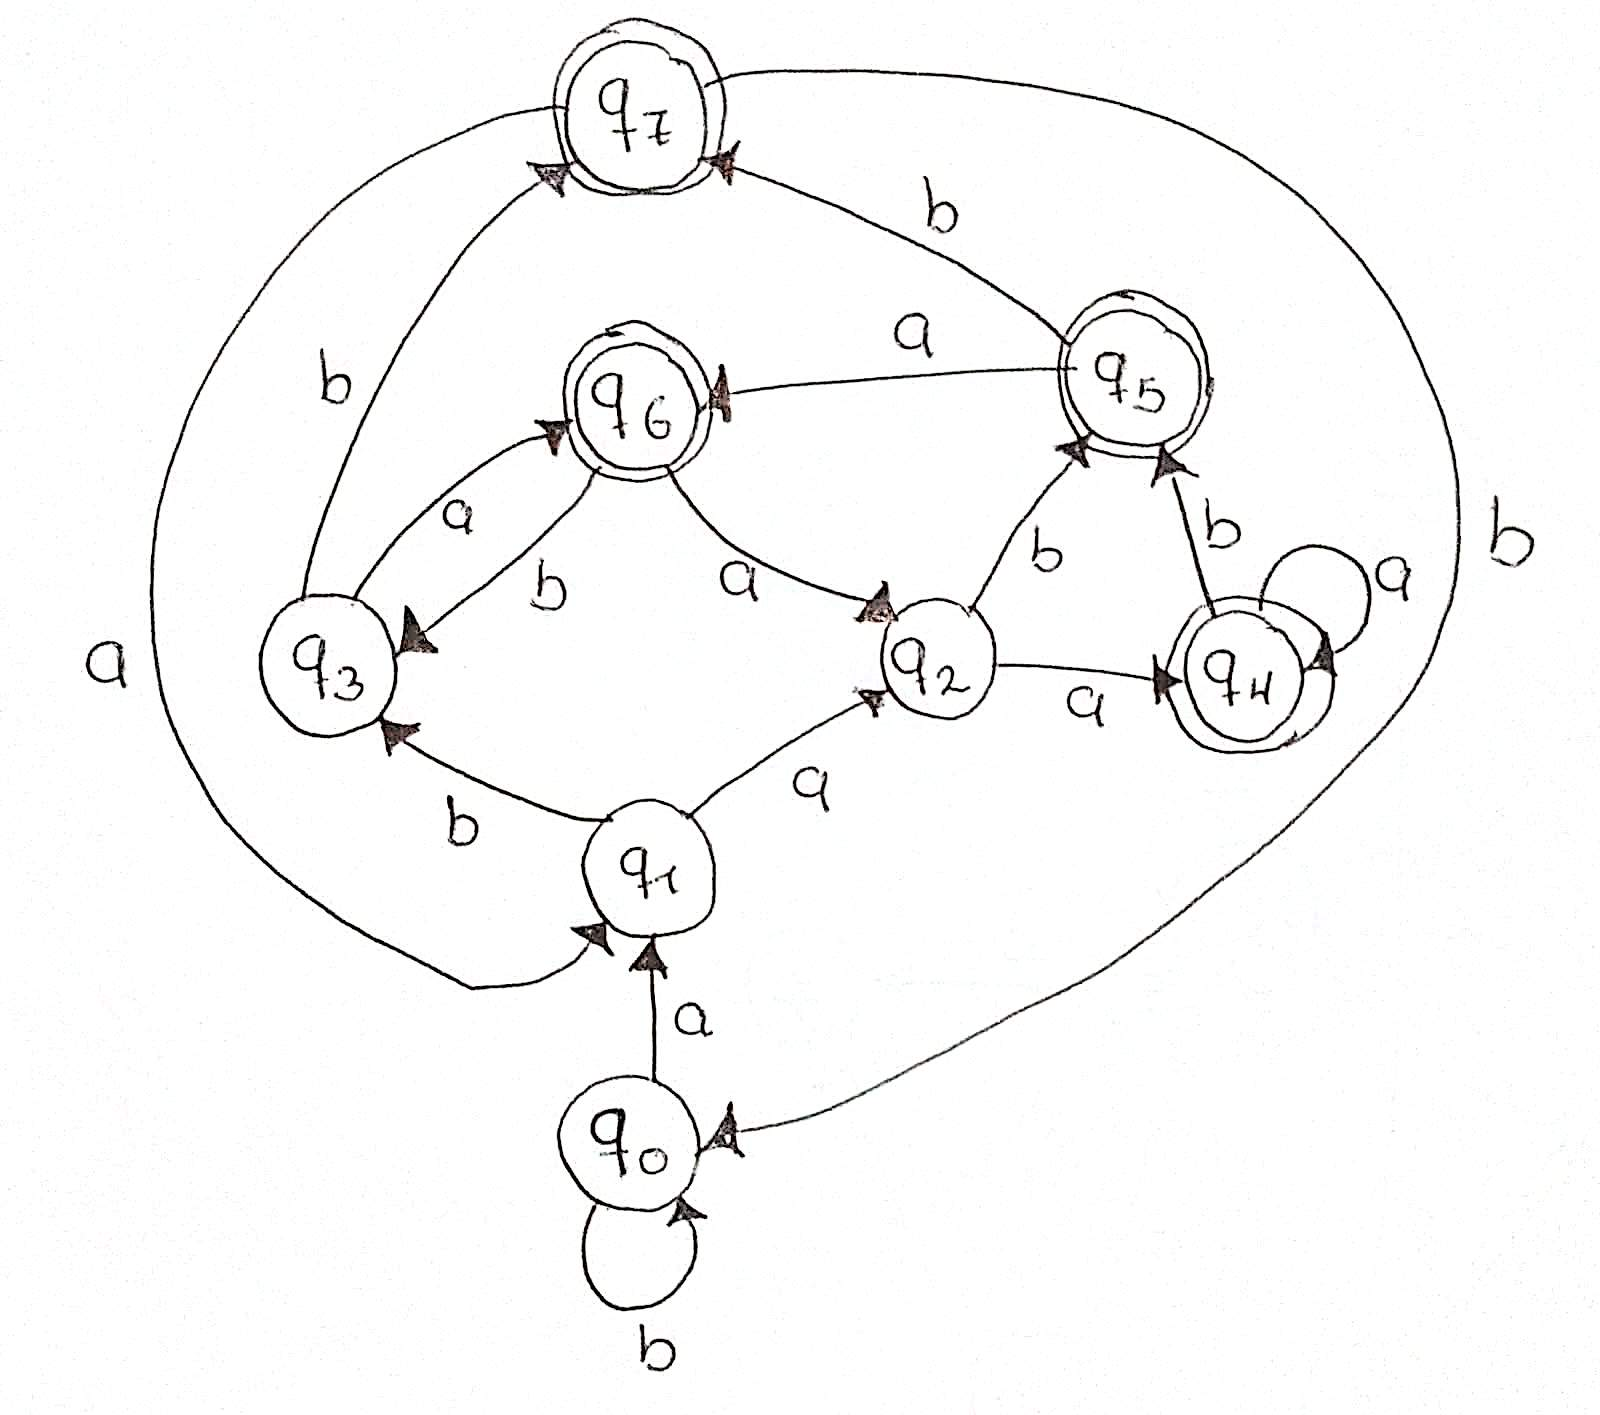
\includegraphics[width=0.6\textwidth]{img.jpg}
      \label{fig:cable-cruzado}
    \end{figure}
    
    \newpage
    
  \item $(a|b)^*a(a|b)(a|b)(a|b)$.

    \subsection*{Elementos Punteados}
    El mismo patrón una vez más, agregando un tercer grupo $(a\mid b)$ al final (por espacio se omite
    el listado de ítems, que es idéntico al de \textit{b)} con un nivel extra.

    \subsubsection*{Tabla de transiciones:}
    \[
    \begin{array}{c|cc}
      & a & b \\ \hline
      \rightarrow q_0 & q_1 & q_0 \\
      q_1 & q_2 & q_3 \\
      q_2 & q_4 & q_5 \\
      q_3 & q_6 & q_7 \\
      q_4 & q_8 & q_9 \\
      q_5 & q_{10} & q_{11} \\
      q_6 & q_{12} & q_{13} \\
      q_7 & q_{14} & q_{15} \\
      {}^*q_8 & q_8 & q_9 \\
      {}^*q_9 & q_{10} & q_{11} \\
      {}^*q_{10} & q_{12} & q_{13} \\
      {}^*q_{11} & q_{14} & q_{15} \\
      {}^*q_{12} & q_4 & q_5 \\
      {}^*q_{13} & q_6 & q_7 \\
      {}^*q_{14} & q_2 & q_3 \\
      {}^*q_{15} & q_1 & q_0
    \end{array}
    \]

    (Omitimos el diagrama gráfico por el número de estados, la tabla es más práctica de leer.)\\

    \medskip
    
    \subsection*{Minimización}

    \subsubsection*{Paso 1. Partición inicial}
    \[
    \alpha = \{q_8,\dots,q_{15}\} \qquad \beta = \{q_0,\dots,q_7\}
    \]

    \subsubsection*{Paso 2. Verificar transiciones dentro de cada grupo}
    \[
    \begin{array}{c|cc}
      \alpha & a & b \\ \hline
      q_8 & \alpha & \alpha \\
      q_9 & \alpha & \alpha \\
      q_{10} & \alpha & \alpha \\
      q_{11} & \alpha & \alpha \\
      q_{12} & \beta & \beta \\
      q_{13} & \beta & \beta \\
      q_{14} & \beta & \beta \\
      q_{15} & \beta & \beta
    \end{array}
    \qquad
    \begin{array}{c|cc}
      \beta & a & b \\ \hline
      q_0 & \beta & \beta \\
      q_1 & \beta & \beta \\
      q_2 & \beta & \beta \\
      q_3 & \beta & \beta \\
      q_4 & \alpha & \alpha \\
      q_5 & \alpha & \alpha \\
      q_6 & \alpha & \alpha \\
      q_7 & \alpha & \alpha
    \end{array}
    \]

    \subsubsection*{Paso 3. Refinar la partición}
    \[
    \alpha = \{q_8,q_9,q_{10},q_{11}\} \quad \beta = \{q_0,q_1,q_2,q_3\} \quad \gamma = \{q_{12},q_{13},q_{14},q_{15}\} \quad \delta = \{q_4,q_5,q_6,q_7\}
    \]

    \subsubsection*{Paso 4. Repetir la verificación con 4 grupos}
    \[
    \begin{array}{c|cc}
      \alpha & a & b \\ \hline
      q_8 & \alpha & \alpha \\
      q_9 & \alpha & \alpha \\
      q_{10} & \gamma & \gamma \\
      q_{11} & \gamma & \gamma
    \end{array}
    \qquad
    \begin{array}{c|cc}
      \gamma & a & b \\ \hline
      q_{12} & \delta & \delta \\
      q_{13} & \delta & \delta \\
      q_{14} & \beta & \beta \\
      q_{15} & \beta & \beta
    \end{array}
    \]
    \[
    \begin{array}{c|cc}
      \beta & a & b \\ \hline
      q_0 & \beta & \beta \\
      q_1 & \beta & \beta \\
      q_2 & \delta & \delta \\
      q_3 & \delta & \delta
    \end{array}
    \qquad
    \begin{array}{c|cc}
      \delta & a & b \\ \hline
      q_4 & \alpha & \alpha \\
      q_5 & \alpha & \alpha \\
      q_6 & \gamma & \gamma \\
      q_7 & \gamma & \gamma
    \end{array}
    \]

    \subsubsection*{Paso 5. Refinar de nuevo (4 $\to$ 8 grupos)}
    \[
    \alpha = \{q_8,q_9\} \quad \varepsilon = \{q_{10},q_{11}\} \quad \gamma = \{q_{12},q_{13}\} \quad \zeta = \{q_{14},q_{15}\}
    \]
    \[
    \beta = \{q_0,q_1\} \quad \eta = \{q_2,q_3\} \quad \delta = \{q_4,q_5\} \quad \theta = \{q_6,q_7\}
    \]

    \subsubsection*{Paso 6. Repetir la verificación con 8 grupos}
    \[
    \begin{array}{c|cc}
      \alpha & a & b \\ \hline
      q_8 & \alpha & \alpha \\
      q_9 & \varepsilon & \varepsilon
    \end{array}
    \quad
    \begin{array}{c|cc}
      \varepsilon & a & b \\ \hline
      q_{10} & \gamma & \gamma \\
      q_{11} & \zeta & \zeta
    \end{array}
    \quad
    \begin{array}{c|cc}
      \gamma & a & b \\ \hline
      q_{12} & \delta & \delta \\
      q_{13} & \theta & \theta
    \end{array}
    \quad
    \begin{array}{c|cc}
      \zeta & a & b \\ \hline
      q_{14} & \eta & \eta \\
      q_{15} & \beta & \beta
    \end{array}
    \]
    \[
    \begin{array}{c|cc}
      \beta & a & b \\ \hline
      q_0 & \beta & \beta \\
      q_1 & \eta & \eta
    \end{array}
    \quad
    \begin{array}{c|cc}
      \eta & a & b \\ \hline
      q_2 & \delta & \delta \\
      q_3 & \theta & \theta
    \end{array}
    \quad
    \begin{array}{c|cc}
      \delta & a & b \\ \hline
      q_4 & \alpha & \alpha \\
      q_5 & \varepsilon & \varepsilon
    \end{array}
    \quad
    \begin{array}{c|cc}
      \theta & a & b \\ \hline
      q_6 & \gamma & \gamma \\
      q_7 & \zeta & \zeta
    \end{array}
    \]

    \subsubsection*{Paso 7. Refinar de nuevo (8 $\to$ 16 grupos)}
    Cada uno de los ocho grupos se separa en dos: se obtienen 16 grupos unitarios, uno por cada estado original.

    \subsubsection*{Paso 8. Conclusión}
    No pueden refinarse más (todos los grupos son unitarios). No existen estados equivalentes: \textbf{el AFD ya era mínimo} (16 estados). La tabla de transiciones mínima coincide exactamente con la original:

    \medskip

    \[
    \begin{array}{c|cc}
      & a & b \\ \hline
      \rightarrow q_0 & q_1 & q_0 \\
      q_1 & q_2 & q_3 \\
      q_2 & q_4 & q_5 \\
      q_3 & q_6 & q_7 \\
      q_4 & q_8 & q_9 \\
      q_5 & q_{10} & q_{11} \\
      q_6 & q_{12} & q_{13} \\
      q_7 & q_{14} & q_{15} \\
      {}^*q_8 & q_8 & q_9 \\
      {}^*q_9 & q_{10} & q_{11} \\
      {}^*q_{10} & q_{12} & q_{13} \\
      {}^*q_{11} & q_{14} & q_{15} \\
      {}^*q_{12} & q_4 & q_5 \\
      {}^*q_{13} & q_6 & q_7 \\
      {}^*q_{14} & q_2 & q_3 \\
      {}^*q_{15} & q_1 & q_0 \\
    \end{array}
    \]

    \medskip
    \noindent
    (Volvemos a omitir el diagrama de transiciones por su tamaño: 16 estados y 32 aristas; la tabla lo especifica por completo.)
  \end{enumerate}
  
  \bigskip

  
%%%%%%%%%%%%%%%%%%%%%%%%%%%%%%%%%%%%%%%%%%
\newpage
%%%%%%%%%%%%%%%%%%%%%%%%%%%%%%%%%%%%%%%%%%

\item La siguiente gramática genera el lenguaje representado por la expresión regular $0^*1(0+1)^*$:
  \[
  S \to A1B
  \]
  \[
  A \to 0A \mid \varepsilon
  \]
  \[
  B \to 0B \mid 1B \mid \varepsilon
  \]
  Obtenga las derivaciones más a la izquierda y más a la derecha de las siguientes cadenas. Por último, obtenga el árbol de gramática o de derivación.
  \begin{enumerate}
  \item $00101$
  \item $1001$
  \item $00011$
  \end{enumerate}
  
  \bigskip

  \subsubsection*{$a)\;\; 00101$}
  \begin{center}
    \noindent
    \begin{minipage}[t]{0.30\textwidth}
      \centering
      \textbf{Izquierda}
      
      \vspace{5pt}
      
      $S \Rightarrow A1B$

      $\Rightarrow 0A1B$

      $\Rightarrow 00A1B$

      $\Rightarrow 00\varepsilon1B$

      $\Rightarrow 001B$

      $\Rightarrow 0010B$

      $\Rightarrow 00101B$

      $\Rightarrow 00101\varepsilon$

      $\Rightarrow \boxed{00101}$
    \end{minipage}
    \hfill
    \vrule
    \hfill
    \begin{minipage}[t]{0.30\textwidth}
      \centering
      \textbf{Derecha}

      \vspace{5pt}

      $S \Rightarrow A1B$

      $\Rightarrow A10B$

      $\Rightarrow A10 1B$

      $\Rightarrow A101\varepsilon$

      $\Rightarrow 0A101\varepsilon$

      $\Rightarrow 00A101\varepsilon$
      
      $\Rightarrow 00\varepsilon101\varepsilon$
      
      $\Rightarrow \boxed{00101}$
    \end{minipage}
    \hfill
    \vrule
    \hfill
    \begin{minipage}[t]{0.30\textwidth}
      \centering
      \textbf{Árbol de derivación}

      \vspace{10pt}

      \begin{forest}
        for tree={
          math content,
          edge={-},
          s sep=8pt,
          l sep=10pt,
          align=center,
        }
        [S
          [A
            [0]
            [A
              [0]
              [A
                [$\varepsilon$]
              ]
            ]
          ]
          [1]
          [B
            [0]
            [B
              [1]
              [B
                [$\varepsilon$]
              ]
            ]
          ]
        ]
    \end{forest}
    \end{minipage}
  \end{center}

  %%%%%%%%%%%%%%%%%%%%%%%%%%%%%%
  
  \subsubsection*{$b)\;\; 1001$}
  \begin{center}
    \noindent
    \begin{minipage}[t]{0.30\textwidth}
      \centering
      \textbf{Izquierda}
      
      \vspace{5pt}
      
      $S \Rightarrow A1B$

      $\Rightarrow \varepsilon1B$

      $\Rightarrow 1B$

      $\Rightarrow 10B$

      $\Rightarrow 100B$

      $\Rightarrow 1001B$

      $\Rightarrow 1001\varepsilon$

      $\Rightarrow \boxed{1001}$
    \end{minipage}
    \hfill
    \vrule
    \hfill
    \begin{minipage}[t]{0.30\textwidth}
      \centering
      \textbf{Derecha}

      \vspace{5pt}

      $S \Rightarrow A1B$

      $\Rightarrow A10B$

      $\Rightarrow A100B$

      $\Rightarrow A1001B$

      $\Rightarrow A1001\varepsilon$

      $\Rightarrow A1001$
      
      $\Rightarrow \varepsilon1001$
      
      $\Rightarrow \boxed{1001}$
    \end{minipage}
    \hfill
    \vrule
    \hfill
    \begin{minipage}[t]{0.30\textwidth}
      \centering
      \textbf{Árbol de derivación}

      \vspace{10pt}

      \begin{forest}
        for tree={
          math content,
          edge={-},
          s sep=8pt,
          l sep=10pt,
          align=center,
        }
        [S
          [A
            [$\varepsilon$]
          ]
          [1]
          [B
            [0]
            [B
              [0]
              [B
                [1]
                [B
                  [$\varepsilon$]
                ]
              ]
            ]
          ]
        ]
    \end{forest}
    \end{minipage}
  \end{center}

  %%%%%%%%%%%%%%%%%%%%%%%%%%%%%%%
  
  \subsubsection*{$c)\;\; 00011$}
  \begin{center}
    \noindent
    \begin{minipage}[t]{0.30\textwidth}
      \centering
      \textbf{Izquierda}
      
      \vspace{5pt}
      
      $S \Rightarrow A1B$

      $\Rightarrow 0A1B$

      $\Rightarrow 00A1B$

      $\Rightarrow 000A1B$

      $\Rightarrow 000\varepsilon1B$

      $\Rightarrow 0001B$

      $\Rightarrow 00011B$

      $\Rightarrow 00011\varepsilon$

      $\Rightarrow \boxed{00011}$
    \end{minipage}
    \hfill
    \vrule
    \hfill
    \begin{minipage}[t]{0.30\textwidth}
      \centering
      \textbf{Derecha}

      \vspace{5pt}

      $S \Rightarrow A1B$

      $\Rightarrow A11B$

      $\Rightarrow A11\varepsilon$

      $\Rightarrow A11$

      $\Rightarrow 0A11$

      $\Rightarrow 00A11$
      
      $\Rightarrow 000A11$

      $\Rightarrow 000\varepsilon11$
      
      $\Rightarrow \boxed{00011}$
    \end{minipage}
    \hfill
    \vrule
    \hfill
    \begin{minipage}[t]{0.30\textwidth}
      \centering
      \textbf{Árbol de derivación}

      \vspace{10pt}

      \begin{forest}
        for tree={
          math content,
          edge={-},
          s sep=8pt,
          l sep=10pt,
          align=center,
        }
        [S
          [A
            [0]
            [A
              [0]
              [A
                [0]
                [A
                  [$\varepsilon$]
                ]
              ]
            ]
          ]
          [1]
          [B
            [1]
            [B
              [$\varepsilon$]
            ]
          ]
        ]
    \end{forest}
    \end{minipage}
  \end{center}
%%%%%%%%%%%%%%%%%%%%%%%%%%%%%%%%%%%%%%%%%%
\newpage
%%%%%%%%%%%%%%%%%%%%%%%%%%%%%%%%%%%%%%%%%%


\item La gramática siguiente genera todas las expresiones regulares sobre el alfabeto de
  letras:
  \[
  \begin{aligned}
    rexp &\to rexp \mid rexp \\
    &\mid rexp\ rexp \\
    &\mid rexp * \\
    &\mid (rexp) \\
    &\mid letra
  \end{aligned}
  \]

  \begin{enumerate}[label=\alph*.]

  \item Muestre que esta gramática es ambigua usando la derivación de $a\mid b\mid c$.

    \textbf{Recordatorio:} una gramática es ambigua si existe al menos una cadena que admite
    dos árboles de derivación distintos.

    \medskip
    \textbf{El problema.} La regla $rexp \to rexp \mid rexp$ no especifica cómo se agrupan los
    operadores $\mid$ cuando hay más de uno seguido. Para la cadena $a\mid b\mid c$ esto puede
    interpretarse como $(a\mid b)\mid c$ \emph{o} como $a\mid(b\mid c)$ (los paréntesis son solo
    para enfatizar el agrupamiento, no forman parte de la cadena).

    \medskip
    \textbf{Derivación Izquierda:} expandimos el $rexp$ más a la izquierda:
    \[
    \begin{aligned}
      rexp &\Rightarrow rexp \mid rexp \\
      &\Rightarrow rexp \mid rexp \mid rexp \\
      &\Rightarrow letra \mid rexp \mid rexp \\
      &\Rightarrow a \mid rexp \mid rexp \\
      &\Rightarrow a \mid letra \mid rexp \\
      &\Rightarrow a \mid b \mid rexp \\
      &\Rightarrow a \mid b \mid letra \\
      &\Rightarrow a\mid b\mid c
    \end{aligned}
    \]
    El su árbol de derivación, el nodo raíz agrupa $(a\mid b)$ como hijo izquierdo, y $c$ como hijo derecho.

    \textbf{Derivación Derecha:} expandimos el $rexp$ más a la derecha:
    \[
    \begin{aligned}
      rexp &\Rightarrow rexp \mid rexp \\
      &\Rightarrow rexp \mid rexp \mid rexp \\
      &\Rightarrow rexp \mid rexp \mid letra \\
      &\Rightarrow rexp \mid rexp \mid c \\
      &\Rightarrow rexp \mid letra \mid c \\
      &\Rightarrow rexp \mid b \mid c \\
      &\Rightarrow letra \mid b \mid c \\
      &\Rightarrow a\mid b\mid c
    \end{aligned}
    \]
    El su árbol de derivación, el nodo raíz agrupa $a$ como hijo izquierdo, y $(b\mid c)$ como hijo derecho.\\

    Ambas derivaciones producen la misma cadena $a\mid b\mid c$, pero con dos árboles de derivación distintos.
    Como existen dos árboles distintos para la misma cadena, \textbf{la gramática es ambigua}.
    El origen del problema es que la regla $rexp \to rexp\mid rexp$ no fija cuál instancia de
    $rexp$ debe expandirse primero cuando el operador se repite.

  \item Vuelva a escribir esta gramática para establecer las precedencias.

    Establecemos la jerarquía de precedencia (de mayor a menor):
    \begin{enumerate}
    \item[1.] $*$\; : mayor precedencia (cierre de Kleene)
    \item[2.] concatenación\; : precedencia intermedia
    \item[3.] $\mid$\; : menor precedencia
    \end{enumerate}

    Introducimos un no terminal por cada nivel, de modo que cada uno solo pueda usar
    operadores de su nivel o de nivel superior. \textbf{Nota de notación:} para no confundir
    el símbolo \emph{literal} $\mid$ de la regex (un terminal, parte de la cadena que se
    reconoce) con el símbolo $\mid$ de \emph{BNF} (que solo separa alternativas de una
    producción), escribimos el terminal en \texttt{|} y dejamos $\mid$ para las alternativas
    de la gramática:
    \[
    \begin{aligned}
      rexp &\to rexp \;\texttt{|}\; concat \mid concat \\
      concat &\to concat\ factor \mid factor \\
      factor &\to factor * \mid atom \\
      atom &\to (rexp) \mid letra
    \end{aligned}
    \]

    \textbf{Verificación.} Con esta gramática, la única derivación posible
    de $a\mid b\mid c$ es:
    \[
    \begin{aligned}
      rexp &\Rightarrow rexp\,\texttt{|}\,concat \\
      &\Rightarrow rexp\,\texttt{|}\,concat\,\texttt{|}\,concat
      \quad\text{(la única forma de generar \texttt{|} es reexpandir el $rexp$ izquierdo)}\\
      &\Rightarrow concat\,\texttt{|}\,concat\,\texttt{|}\,concat
      \quad\text{(ya no se puede seguir, usamos la base $rexp\to concat$)}\\
      &\Rightarrow^{*} a\,\texttt{|}\,concat\,\texttt{|}\,concat
      \quad(concat\Rightarrow factor\Rightarrow atom\Rightarrow letra\Rightarrow a)\\
      &\Rightarrow^{*} a\,\texttt{|}\,b\,\texttt{|}\,concat \;\Rightarrow^{*}\; a\,\texttt{|}\,b\,\texttt{|}\,c
    \end{aligned}
    \]
    En ningún paso hubo elección de \emph{cuál} $rexp$ expandir para generar el siguiente
    \texttt{|}, como la recursión solo existe del lado izquierdo ($rexp \to rexp\,\texttt{|}\,concat$),
    el único árbol posible agrupa como $(a\mid b)\mid c$. Al no existir una segunda derivación
    con árbol distinto, \textbf{la gramática ya no es ambigua}.
    
    \bigskip
    
  \item ¿Qué asociatividad da su respuesta en el inciso b para los operadores binarios?
    Explique su respuesta.
    
    Los operadores binarios de esta gramática son $\mid$ (el literal) y la concatenación. En
    ambos casos la recursión aparece del lado \textbf{izquierdo} del no terminal:
    \[
    rexp \to rexp\,\texttt{|}\,concat \qquad\qquad concat \to concat\ factor
    \]
    Esto obliga a que, al derivar una cadena con el operador repetido, el símbolo más
    reciente quede siempre agrupado con lo ya generado a la izquierda (justo como se vio en
    la verificación del inciso b). Por lo tanto, \textbf{ambos operadores binarios son
      asociativos por la izquierda}.
    
    \emph{(Si en vez de esto quisiéramos asociatividad por la derecha, la recursión debería
    ir del lado derecho, por ejemplo $rexp \to concat\,\texttt{|}\,rexp$.)}
  \end{enumerate}
  
  
%%%%%%%%%%%%%%%%%%%%%%%%%%%%%%%%%%%%%%%%%%
\newpage
%%%%%%%%%%%%%%%%%%%%%%%%%%%%%%%%%%%%%%%%%%

\item Considere la gramática siguiente:
  \[
  E \to E + T \mid T
  \]
  \[
  T \to T * F \mid F
  \]
  \[
  F \to (E) \mid n
  \]

  \begin{enumerate}[label=\alph*.]

  \item Traduzca la gramática a EBNF.

    \bigskip
    
    Cada regla tiene la forma de recursión izquierda $X \to X\,\alpha \mid \beta$, donde $\beta$ aparece una
    sola vez y $\alpha$ se puede repetir cero o más veces después. En \textbf{EBNF} esto se expresa directamente
    con la notación de repetición $\{\ldots\}$ (cero o más veces), sin necesidad de recursión:
    \[
    X \to X\,\alpha \mid \beta \qquad \Longrightarrow \qquad X \to \beta\,\{\alpha\}
    \]

    Aplicando esto a cada regla:
    \[
    \begin{aligned}
      E &\to T\,\{+\,T\} \\
      T &\to F\,\{*\,F\} \\
      F &\to (E) \mid n
    \end{aligned}
    \]

    $F$ no tiene recursión izquierda, así que se queda igual.

    \bigskip
    
  \item Dibuje diagramas de sintaxis para la EBNF del inciso a.
    
    \bigskip
    
    \textbf{Diagrama para $E \to T\,\{+\,T\}$}
    \begin{center}
      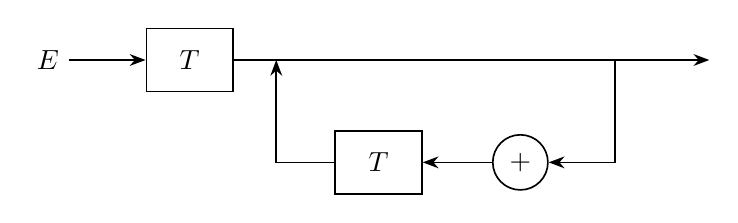
\begin{tikzpicture}[>=Stealth, semithick,
          nonterm/.style={draw, rectangle, minimum width=1.1cm, minimum height=0.8cm},
          term/.style={draw, circle, minimum size=0.7cm, inner sep=1pt}
        ]
        \node (E) at (-2.0,0) {$E$};
        \node[nonterm] (T1) at (-0.2,0) {$T$};
        \coordinate (branch) at (5.2,0);
        \coordinate (salida) at (6.4,0);
        \coordinate (merge)  at (0.9,0);
        
        \node[term]    (mas) at (4.0,-1.3) {$+$};
        \node[nonterm] (T2)  at (2.2,-1.3) {$T$};
        
        % camino principal
        \draw[->] (E) -- (T1.west);
        \draw     (T1.east) -- (branch);
        \draw[->] (branch) -- (salida);
        
        % ciclo de repetición { + T }
        \draw[->] (branch) |- (mas.east);
        \draw[->] (mas.west) -- (T2.east);
        \draw[->] (T2.west) -| (merge);
      \end{tikzpicture}
    \end{center}
    
    \bigskip
    \bigskip
    
    \textbf{Diagrama para $T \to F\,\{*\,F\}$}
    \begin{center}
      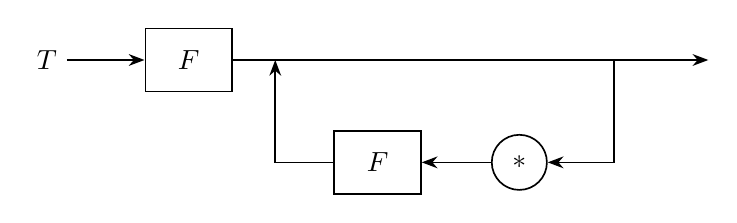
\begin{tikzpicture}[>=Stealth, semithick,
          nonterm/.style={draw, rectangle, minimum width=1.1cm, minimum height=0.8cm},
          term/.style={draw, circle, minimum size=0.7cm, inner sep=1pt}
        ]
        \node (Tin) at (-2.0,0) {$T$};
        \node[nonterm] (F1) at (-0.2,0) {$F$};
        \coordinate (branch) at (5.2,0);
        \coordinate (salida) at (6.4,0);
        \coordinate (merge)  at (0.9,0);
        
        \node[term]    (star) at (4.0,-1.3) {$*$};
        \node[nonterm] (F2)   at (2.2,-1.3) {$F$};
        
        \draw[->] (Tin) -- (F1.west);
        \draw     (F1.east) -- (branch);
        \draw[->] (branch) -- (salida);
        
        \draw[->] (branch) |- (star.east);
        \draw[->] (star.west) -- (F2.east);
        \draw[->] (F2.west) -| (merge);
      \end{tikzpicture}
    \end{center}
    
    \bigskip
    \bigskip
    
    \textbf{Diagrama para $F \to (E) \mid n$} (alternativa, no ciclo)
    \begin{center}
      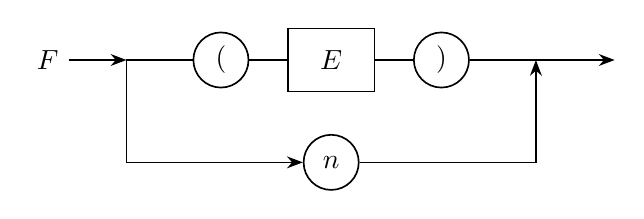
\begin{tikzpicture}[>=Stealth, semithick,
          nonterm/.style={draw, rectangle, minimum width=1.1cm, minimum height=0.8cm},
          term/.style={draw, circle, minimum size=0.7cm, inner sep=1pt}
        ]
        \node (Fin) at (0,0) {$F$};
        \coordinate (split) at (1.0,0);
        \node[term]    (lp) at (2.2,0)  {$($};
        \node[nonterm] (E)  at (3.6,0)  {$E$};
        \node[term]    (rp) at (5.0,0)  {$)$};
        \coordinate (join)  at (6.2,0);
        \coordinate (salida) at (7.2,0);
        
        \node[term] (n) at (3.6,-1.3) {$n$};
        
        % rama superior: ( E )
        \draw[->] (Fin) -- (split);
        \draw     (split) -- (lp.west);
        \draw     (lp.east) -- (E.west);
        \draw     (E.east) -- (rp.west);
        \draw     (rp.east) -- (join);
        \draw[->] (join) -- (salida);
        
        % rama inferior: n
        \draw[->] (split) |- (n.west);
        \draw[->] (n.east) -| (join);
      \end{tikzpicture}
    \end{center}
    
  \end{enumerate}
  
\end{enumerate}

\end{document}
